\documentclass{report}

%----------------- packages include list ----------------
\usepackage{graphicx}
\usepackage{graphics}
\usepackage[doublespacing]{setspace}
\usepackage{wrapfig,booktabs}
\usepackage{subfigure}
\usepackage{amsmath,varwidth,array,ragged2e,amssymb}
\usepackage{amsfonts}
\usepackage{amsbsy}
\usepackage{float}
\usepackage{graphicx}
\usepackage{placeins}
\usepackage{mathtools}
\usepackage{tikz}
\usepackage{url}
\usepackage{siunitx}
\usepackage[linesnumbered,ruled]{algorithm2e}
\usepackage{paralist}

%----------------------------------------------------------------------------------------
%	LISTINGS
%----------------------------------------------------------------------------------------
\usepackage{verbatim}
\usepackage{xcolor}
\definecolor{bgcolor}{rgb}{0.98,0.98,0.98}
\definecolor{light-gray}{gray}{0.95}
\usepackage{listings}
\lstset{language=C}
\lstset{
  basicstyle=\footnotesize\ttfamily,
  breaklines=true,
  showstringspaces=false,
  numbers=none,
  backgroundcolor=\color{white},
  commentstyle=\color{red},
  keywordstyle=\color{black}\bfseries,
  keywordstyle=[1]\color{black},   % cyan or teal can also be a good choice, use \bfseries for bold
  frame=none,                     % adds a frame around the code
  %xleftmargin=\parindent,
  tabsize=2,                      % sets default tabsize to 2 spaces
  captionpos=b,                   % sets the caption-position to bottom
  morekeywords=[1]{               % if you want to add more keywords to the set
    MODELTYPE,
    __CALCL_MODEL_3D,
    MODEL_2D,
    MODEL_3D,
    CALCLcontext,
    CALCLdevice,
    CALCLkernel,
    CALCLManager,
    CALCLmem,
    CALCLModel2D,
    CALCLModel3D,
    CALCLprogram,
    CAL_CUSTOM_NEIGHBORHOOD_2D,
    CAL_CUSTOM_NEIGHBORHOOD_3D,
    CAL_FALSE,
    CALGL_DATA_TYPE_DYNAMIC,
    CALGL_DRAW_MODE_FLAT,
    CALGL_DRAW_MODE_SURFACE,
    CALGL_INFO_BAR_ORIENTATION_VERTICAL,
    CALGL_TYPE_INFO_USE_CURRENT_COLOR,
    CALGL_TYPE_INFO_USE_RED_YELLOW_SCALE,
    CALGL_TYPE_INFO_USE_NO_COLOR,
    CALGL_TYPE_INFO_COLOR_DATA,
    CALGL_TYPE_INFO_NORMAL_DATA,
    CALGL_TYPE_INFO_VERTEX_DATA,
    CALGL_TYPE_INFO_USE_CONST_VALUE,
    CALGL_TYPE_INFO_USE_DEFAULT,
    CALGL_TYPE_INFO_USE_RED_SCALE,
    CALGL_DATA_TYPE_STATIC,
    CALGLRun2D,
    CALGLRun3D,
    CALGLDrawModel2D,
    CALGLDrawModel3D,
    CAL_HEXAGONAL_NEIGHBORHOOD_2D,
    CAL_HEXAGONAL_NEIGHBORHOOD_ALT_2D,
    CAL_MOORE_NEIGHBORHOOD_2D,
    CAL_MOORE_NEIGHBORHOOD_3D,
    CAL_NO_OPT,
    CAL_OPT_ACTIVE_CELLS,
    CAL_RUN_LOOP,
    CAL_SPACE_FLAT,
    CAL_SPACE_TOROIDAL,
    CAL_TRUE,
    CAL_UPDATE_EXPLICIT,
    CAL_UPDATE_IMPLICIT,
    CAL_VON_NEUMANN_NEIGHBORHOOD_2D,
    CAL_VON_NEUMANN_NEIGHBORHOOD_3D,
    calAddActiveCell2D,
    calAddActiveCell3D,
    calAddActiveCellX2D,
    calAddActiveCellX3D,
    calAddElementaryProcess2D,
    calAddElementaryProcess3D,
    calAddSingleLayerSubstate2Db,
    calAddSingleLayerSubstate2Di,
    calAddSingleLayerSubstate2Dr,
    calAddSingleLayerSubstate3Db,
    calAddSingleLayerSubstate3Di,
    calAddSingleLayerSubstate3Dr,
    calAddSubstate2Db,
    calAddSubstate2Di,
    calAddSubstate2Dr,
    calAddSubstate3Db,
    calAddSubstate3Di,
    calAddSubstate3Dr,
    calAddActiveCell2D,
    calAddActiveCellX2D,
    calAddActiveCell3D,
    calAddActiveCellX3D,
    calApplyElementaryProcess2D,
    calApplyElementaryProcess3D,
    CALbyte,
    calclAddActiveCell2D,
    calclAddActiveCellX2D,
    calclAddElementaryProcess2D,
    calclAddElementaryProcess3D,
    calclAddReductionSum2Di,
    calclAddStopConditionFunc2D,
    calclAddStopConditionFunc3D,
    calclAddSteeringFunc2D,
    calclAddSteeringFunc3D,
    calclCreateBuffer,
    calclCreateContext,
    calclCreateManager,
    calCADef2D,
    calCADef3D,
    calclCADef2D,
    calclCADef3D,
    calclFinalizeManager,
    calclFinalize2D,
    calclFinalize3D,
    calclGet2Db,
    calclGet3Db,
    calclGet2Di,
    calclGet3Di,
    calclGet2Dr,
    calclGet3Dr,
    calclGetX2Db,
    calclGetX2Di,
    calclGetX2Dr,
    calclGetX3Db,
    calclGetX3Di,
    calclGetX3Dr,
    calclGetDevice,
    calclGetSum2Di,
    calclGlobalRow,
    calclGlobalColumn,
    calclGlobalSlice,
    calclInitializePlatforms,
    calclInitializeDevices,
    calclLoadProgram2D,
    calclLoadProgram3D,
    calclLocalRow,
    calclLocalColumn,
    calclLocalSlice,
    calclGetKernelFromProgram,
    calclGetRows,
    calclGetColumns,
    calclGetSlices,
    calclgGetByteSubstatesNum,
    calclGetIntSubstatesNum,
    calclGetRealSubstatesNum,
    calclGetCurrentByteSubstates,
    calclGetCurrentIntSubstates,
    calclGetCurrentRealSubstates,
    calclGetNextByteSubstates,
    calclGetNextIntSubstates,
    calclGetNnextRealSubstates,
    calclGetNeighborhood,
    calclGetNeighborhoodID,
    calclGetNeighborhoodSize,
    calclGetBoundaryCondition,
    calclGetPlatformAndDeviceFromStdIn,
    calclRemoveActiveCell2D,
    calclRemoveActiveCell3D,
    calclRun2D,
    calclRun3D,
    calclRunStop,
    calclSetKernelArg2D,
    calclSetKernelArg3D,
    calclThreadCheck2D,
    calclThreadCheck2D,
    calclSet2Db,
    calclSet3Db,
    calclSet2Di,
    calclSet3Di,
    calclSet2Dr,
    calclSet3Dr,
    calclActiveThreadCheck2D,
    calclActiveThreadCheck3D,
    CALDrawModel2D,
    CALDrawModel3D,
    calFinalize2D,
    calFinalize3D,
    calGet2Db,
    calGet2Di,
    calGet2Dr,
    calGet3Db,
    calGet3Di,
    calGet3Dr,
    calGetX2Db,
    calGetX2Di,
    calGetX2Dr,
    calGetX3Db,
    calGetX3Di,
    calGetX3Dr,
    calglAdd2Db,
    calglAdd3Db,
    calglAdd2Di,
    calglAdd3Di,
    calglAdd2Dr,
    calglAdd3Dr,
    calglColor2D,
    calglColor3D,
    calglDefDrawModel2D,
    calglDefDrawModel3D,
    calglDefDrawModelCL2D,
    calglDefDrawModelCL3D,
    calglDisplayDrawJBound2D,
    calglHideDrawJBound2D,
    calglInfoBar2Dr,
    calglInitViewer,
    calglMainLoop2D,
    calglMainLoop3D,
    calglRelativeInfoBar2Dr,
    calglRelativeInfoBar3Dr,
    calglRunCLDef2D,
    calglRunCLDef3D,
    calglSetDisplayStep,
    calglSetHeightOffset2D,
    calglSetHeightOffset3D,
    calInit2Db,
    calInit2Di,
    calInit2Dr,
    calInit3Db,
    calInit3Di,
    calInit3Dr,
    calInitSubstate2Db,
    calInitSubstate2Di,
    calInitSubstate2Dr,
    calInitSubstate3Db,
    calInitSubstate3Di,
    calInitSubstate3Dr,
    CALint,
    calLoadSubstate2Db,
    calLoadSubstate2Di,
    calLoadSubstate2Dr,
    calLoadSubstate3Db,
    calLoadSubstate3Di,
    calLoadSubstate3Dr,
    CALModel2D,
    CALModel3D,
    CALNeighborhood2D,
    CALNeighborhood3D,
    CALOptimization,
    CALParameterb,
    CALParameteri,
    CALParameterr,
    CALreal,
    calRemoveActiveCell2D,
    calRemoveActiveCell3D,
    CALRun2D,
    CALRun3D,
    calRun2D,
    calRun3D,
    calRunAddGlobalTransitionFunc2D,
    calRunAddGlobalTransitionFunc3D,
    calRunAddInitFunc2D,
    calRunAddInitFunc3D,
    calRunAddSteeringFunc2D,
    calRunAddSteeringFunc3D,
    calRunAddStopConditionFunc2D,
    calRunAddStopConditionFunc3D,
    calRunDef2D,
    calRunDef3D,
    calRunInitSimulation2D,
    calRunInitSimulation3D,
    calRunFinalize2D,
    calRunFinalize3D,
    calRunFinalizeSimulation2D,
    calRunFinalizeSimulation3D,
    calSaveSubstate2Db,
    calSaveSubstate2Di,
    calSaveSubstate2Dr,
    calSaveSubstate3Db,
    calSaveSubstate3Di,
    calSaveSubstate3Dr,
    calSet2Db,
    calSet2Di,
    calSet2Dr,
    calSet3Db,
    calSet3Di,
    calSet3Dr,
    calSetX2Db,
    calSetX2Di,
    calSetX2Dr,
    calSetX3Db,
    calSetX3Di,
    calSetX3Dr,
    calSetCurrent2Db,
    calSetCurrent2Di,
    calSetCurrent2Dr,
    calSetCurrent3Db,
    calSetCurrent3Di,
    calSetCurrent3Dr,
    CALSpaceBoundaryCondition,
    CALSubstate2Db,
    CALSubstate2Di,
    CALSubstate2Dr,
    CALSubstate3Db,
    CALSubstate3Di,
    CALSubstate3Dr,
    calUpdateActiveCells2D,
    calUpdateSubstate2Db,
    calUpdateSubstate2Di,
    calUpdateSubstate2Dr,
    calUpdate2D,
    calUpdate3D,
    CALUpdateMode,
    }
}



\usetikzlibrary{positioning,chains,fit,shapes,calc, matrix}
%--------------------- Commands ---------------------
\newcommand*\circled[1]{\tikz[baseline=(char.base)]{
            \node[shape=circle,draw,inner sep=0.3pt] (char) {#1};}}
\newcommand*{\ArrowLength}{2.0em}%
\newcommand*{\MyRightArrow}[1][]{%
    \tikz [-stealth, red, yshift=0.5ex, baseline] 
        \draw [-stealth, #1] (0,0) -- (\ArrowLength,0) ;
}%
%--------------------- begin document ---------------------
\begin{document}

\title{Phd Thesis}
\author{Davide Spataro}

\maketitle


\pagestyle{plain}
\setcounter{tocdepth}{c5}
%\setstretch{1.05}

\addcontentsline{toc}{section}{\listfigurename}
\addcontentsline{toc}{section}{\listtablename}
\tableofcontents


% $Log: abstract.tex,v $ Revision 1.1  93/05/14  14:56:25  starflt Initial
% revision  Revision 1.1  90/05/04  10:41:01  lwvanels Initial revision   % The
% text of your abstract and nothing else (other than comments) goes here.
% % It will be single-spaced and the rest of the text that is supposed to go on
% % the abstract page will be generated by the abstractpage environment.  This %
% file should be \input (not \include 'd) from cover.tex.
\hfill \\
\textit{\textbf{English}}   \hfill \\
\hfill \\
 In
this thesis, a parallel version of the model SCIARA-fv3\cite{Spataro2010} was
designed and implemented using General-Purpose Computation with Graphics
Processing Units (GPGPU) and specifically, by adopting the NVIDIA Compute
Unified Device Architecture (CUDA)\cite{NvidiaprogGuide} framework in order to
improve the overall execution time. It involves the design and the application
of strategies that allow to avoid incorrect computation results due to race
conditions of any type and at the same time to achieve the best performance and
occupancy of the underlying available hardware. Carried out experiments show
that significant performance improvement in terms of speedup are achieved also
thanks to some original optimizations strategies adopted, confirming the
validity of graphics hardware as an alternative to much more expensive solutions
for the simulation of cellular automata models.
\hfill \\
\begin{center}
\line(1,0){350} \hfill \\
\end{center}
\hfill \\
\hfill \\
\textit{\textbf{Italian}}   \hfill \\
\hfill \\


In questo lavoro di tesi ho progettato ed implementato una versione parallela
del modello numero SCIARA-fv3\cite{Spataro2010} utilizzando le schede grafiche
per il calcolo general-purpose (General Purpose Computation with Graphics
Processing Units - GPGPU), adottando il  Compute Unified Device Architecture (CUDA)\cite{NvidiaprogGuide} framework
di NVIDIA con lo scopo di migliorare i tempi di esecuzione complessivi.
Questo ha comportato il design prima, e l'applicazione vera e propria poi, di
strategie che permettessero sia di evitare errori dovuti a race-conditions di
qualsiasi tipo che di raggiungere gli speedups migliori con l'hardware a
disposizione. Gli esperimenti effettuati mostrano significativi miglioramenti
nelle performance in termini di speedup grazie anche all'utilizzo di alcune stragie d'ottimizzazione nuove,
confermando la validit\`a dell'uso di processori grafici come alternativa a
soluzioni hardware per la parallelizzazione di modelli ad
automi cellulari molto pi\`u costose.




%%*******************************************************************************
%*********************************** First Chapter *****************************
%*******************************************************************************

\chapter{Getting started}  %Title of the First Chapter

\include{CA_FDM/ca}
%*******************************************************************************
%***************************** Finite difference Chapter ***********************
%*******************************************************************************

\chapter{Finite Difference Method}

%------------------Introduction-------------------------------
\section{Introduction}
The finite difference approximation for derivativatives is one of the simplest oldest method to solve differential equations numerically. It was used since 1768 by \textit{L. Euler} to solve one dimensional problem and extended by \textit{C. Runge} to two dimension in 1910 ca. Since the advent of computers in 1950 ca. FDM  popularity skyrocketed and during the last five decades theoretical results have been obtained regarging stability, convergence and other of its properties.



    The general idea behind FDM is that the differential operator is approximated by replacing the derivatived using difference quotients, which are linear combination of function values at the grid points). In order to do so the space and time domain are \textit{partitioned} in a grid like fashion and approximated solutions are computed only for those discrete grid points. The numerical solution is known only at a finite number of points in the physical domain.
    Figure \ref{fig:schematic_repr_fdm} is a schematic representation of how FDM are used to obtain a numerical solution.
    \begin{figure}
    \centering
    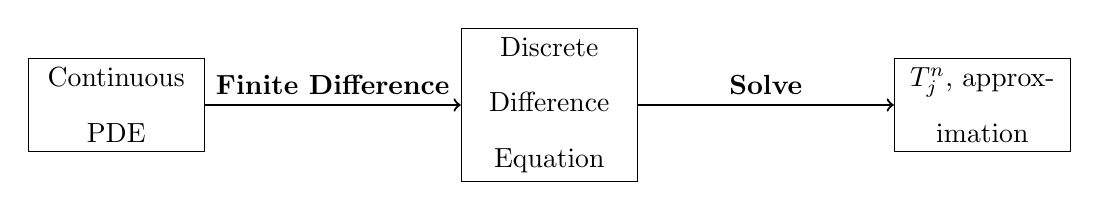
\begin{tikzpicture}

    \node[draw, text centered,text width=2cm] (1) at (0,0) {Continuous PDE};
    \node[draw, text centered,text width=2cm] (2) at (5.5,0) {Discrete Difference Equation};
    \node[draw, text centered,text width=2cm] (3) at (11,0) {$T_j^n$, approximation};

\draw[thick,->] (1) -- (2) node[midway,sloped,above,rotate=0] {\textbf{Finite Difference}};
\draw[thick,->] (2) -- (3) node[midway,sloped,above,rotate=0] {\textbf{Solve}};
\end{tikzpicture}
    \caption{Relationship between continuous and discrete problems.}
    \label{fig:schematic_repr_fdm}
\end{figure}
    
    The error, between the numerical solution and the exact solution is determined by the difference formula utilized and is commonly refeered as \textit{truncation}\footnote{The term truncation comes from the fact that a finite difference quotient is a truncation of the Taylor expansion.} or \textit{discretization} error.  Increasing the resoution of the grid increases the accuracy of the numerical solution since the error associated with the finite difference formulas depends on the distance between grid points.
    
        
    Depending on how the derivatives are approximated, explicit or implicit FDM schemes are
    obtained. When forward difference formulas are considered, the
    resulting difference equation is generally expressed in terms of
    an explicit recurrence formula, while backward difference formulas
    generally lead to implicit recurrence formulas involving unknown
    values, and therefore require the solution of a linear system to
    obtain the new state of the system at each grid point.
    
    
     %------------------Finite difference Formulas-------------------------------
    \section{Finite difference formulas}


    
    Difference formulas can be derived from Tailor's expansion of $T^n_{j+1}$ in terms of $T^n_{j}$ and its derivatives as:
    
    \begin{equation}
    T^n_{j+1} = T^n_{j} +
    \frac{\partial T(t,x)}{\partial x}\bigg\rvert^n_j \Delta x +
    \frac{1}{2!}  \frac{\partial^2 T(t,x)}{\partial x^2}\bigg\rvert^n_j \Delta x^2 + \ldots + 
     \frac{1}{k!}  \frac{\partial^k T(t,x)}{\partial x^k}\bigg\rvert^n_j \Delta x^k + \ldots
     \label{eq:taylorexp1}
    \end{equation}
    
    If series is truncated after the second term ($k=1$) and solving for $\frac{\partial T(t,x)}{\partial x}$ the following is obtained:
    
    \begin{equation}
    \frac{\partial T(t,x)}{\partial x}  = \frac{T^n_{j+1} - T^n_{j}}{\Delta x}
    \label{eq:fdmforward}
    \end{equation}
    
    Equation \ref{eq:fdmforward} is called fist \textbf{forward} finite difference approximation. Other approximations are possible and are easilby obtainable by expanding different points of the grids and using more points from the expansion.
    
    \textbf{Backward} finite difference quotient can be obtained from the Taylor's expansions of    
        \begin{equation}
    T^n_{j-1} = T^n_{j} - 
    \frac{\partial T(t,x)}{\partial x}\bigg\rvert^n_j \Delta x +
    \frac{1}{2!}  \frac{\partial^2 T(t,x)}{\partial x^2}\bigg\rvert^n_j \Delta x^2 + \ldots + 
     \frac{1}{k!}  \frac{\partial^k T(t,x)}{\partial x^k}\bigg\rvert^n_j \Delta x^k + \ldots
     \label{eq:taylorexp2}
    \end{equation}
    
    which can be rearranged in the following manner
        \begin{equation}
    \frac{\partial T(t,x)}{\partial x}  = \frac{T^n_{j} - T^n_{j-1}}{\Delta x}
    \label{eq:fdmfbackward}
    \end{equation}
    
   The same approach can be used to derive approximation for higher order derivatives.
   For example equation \ref{eq:fdmcentral}, known called \textbf{central difference formula}, is an approximation for the second order derivative and can be obtained retaining the firsts four terms in both equations \ref{eq:taylorexp1} and \ref{eq:taylorexp2} and adding the resulting expression:
   
    \begin{equation}
		\frac{\partial^2 T(t,x)}{\partial x^2} = \frac{T^n_{j+1}- 2T^n_{j} + T^n_{j-1}}{\Delta x^2}
		\label{eq:fdmcentral}
    \end{equation}
    
    Figure \ref{fig:geometrical_intepretation} show how finite difference formulas can be interpreted geometrically.
    \begin{figure}
\centering
\includegraphics[scale=0.3]{./images/CA_FDM/geometrical_interpretation_fd}
\label{fig:geometrical_intepretation}
\caption{Explicit FDM discretization for the 1D heat conduction problem}\label{torus}
\end{figure} 
    
    %------------------HEAT Equation-------------------------------
    \section{Heat Equation}
        As an example a simple FDM scheme for an initial-boundary condition problem for the heat conduction problem is derived. 
    
\begin{equation}
    \frac{\partial T(t,x)}{\partial t}= k\frac{\partial^2
      T(t,x)}{\partial x^2}
      \label{eq:heatconduction}
\end{equation}
 
    where $0 \leq t \leq L$ and $0 \leq x \leq
    M$. 
 In order to construct a FD approximation for equation \ref{eq:heatconduction} 
 
 \begin{enumerate}
 
 \item Both space and time domain are partitioned into a finite grid as follows:
    
    \begin{equation}
    		x_j = j\Delta x, \: j = 0,1,\ldots,M,\;\Delta x = \frac{1}{M}
    \end{equation}

 \begin{equation}
    		t_n = n\Delta t, \: n = 0,1,\ldots,L,\; \Delta t= \frac{1}{L}
    \end{equation}  
    
 \item  First and second order derivative appearing in \ref{eq:heatconduction} are substituted by forward and central difference formulas respectively leading to (see Figure  \ref{fig:fdmheatequationstencil}):
 
 \begin{equation}
  \frac{T^n_{j+1} - T^n_{j}}{\Delta x} = k \frac{T^n_{j+1}- 2T^n_{j} + T^n_{j-1}}{\Delta x^2}
 \label{eq:discretizedheatequation}
 \end{equation}
 
 \item Equation \ref{eq:heatconduction} is evaluated at grid point $(n\Delta t, j \Delta x)$ 
    
\end{enumerate}    
    
\begin{figure}
\centering
\includegraphics[scale=0.5]{./images/CA_FDM/heatstencil}
\label{fig:fdmheatequationstencil}
\caption{Explicit FDM discretization for the 1D heat conduction problem}\label{torus}
\end{figure}    
    
\begin{figure}
\centering
\includegraphics[scale=0.3]{./images/CA_FDM/fdmgrid}
\caption{1D heat equation FDM grid space and time partitioning.}\label{torus}
\end{figure}

Solution to equation \ref{eq:heatconduction} requires the specification of boundary conditions at $t=0$ and $x=0$ and $x=M$.
In this example the temperature in the interior of the domain is assumed to be $0$ i.e. and edges in the $x$ dimension are assumed to be source of constant heat i.e. $T(0, 0<x<M)$,  $T(t,0)=100$, $T(t,M)=100$.
         
    $h = \Delta x = 0.2$ and $\Delta t = 0.01$ with initial
    conditions $T(0, 0 < x < M) = 0$ and boundary conditions $T(0,x=0)
    = 100 \: , u(0,x=L) =100$. Note that, assuming $k=1$, the values
    assigned to the spatial and temporal steps satisfy the von Neumann
    stability analysis. In fact, $\frac{k \Delta t}{\Delta x^2} = 1/4
    \leq 1/2$.
   
        In this example, a one-dimensional cellular space $R$
    can be used (cf. Figure \ref{fig:cellularspaces}a) to model the
    $10$ grid points $i$ $(i = 0, 1, ...,9)$, while the values that
    the generic cell can assume are simply represented by the $Q = [0,
      100] \subset \mathbb{R}$ substate. By using the forward
    difference formula for the first order derivative and the central
    one for the second order, the following explicit recurrence scheme
    is obtained:
    $$ T_i^{t+1} = T_i^t + k \Delta t \frac{T_{i+1}^t - 2T_i^t +
      T_{i-1}^t}{\Delta x^2}
    $$ denoting that the value of the temperature at the grid point
    $i$ at the time step $t+1$ is a function of the (known) values
    assumed by $T$ at the $i-1$, $i$ and $i+1$ grid points at the
    (previous) time step $t$. Thus, the one dimensional radious-one $X
    = \{-1, 0, 1\}$ neighburhood pattern can be adopted (cf. Figure
    \ref{fig:1Dneighborhood}a) and an elementary process used to
    implement the above recurrence scheme. The explicit formulation of
    the FDM one-dimensional heat conduction model can be therefore
    expressed in terms of the XCA formalism as:

    $$ FDM_{heat} = <R,\Gamma,X,Q,P,\sigma,\gamma>$$

    \noindent where:

    \begin{itemize}

    \item $R = \{0,1,...,9\}$ is the one-dimensional cellular space,
      representing the integer coordinates of the cells of the
      computational domain (cf. Figure \ref{fig:cellularspaces}a).

    \item $\Gamma = \{0, 9\} \subset R$ is the region identifying the
      boundary of the computational domain.


    \item $X = \{-1, 0, 1\}$ is the geometrical pattern defining the
      neighborhood relationship (cf. Figure
      \ref{fig:1Dneighborhood}a).

    \item $Q = [0, 100] \subset \mathbb{R}$ is the set of cell's
      states used to express the temperature values at the grid
      points.

    \item $P = \{k = 1, \Delta t = 0.01, \Delta x = 0.2\}$ is the set
      of the FDM model parameters.
      
    \item $\sigma : Q^3 \rightarrow Q$ is the cell's transition
      function, which implements the explicit recurrence FDM scheme.

    \item $\gamma: Q^{|\Gamma|} \rightarrow Q^{|\Gamma|} \times
      \mathbb{R}$ is the global steering function, used to apply the
      boundary conditions at each computational step.

    \end{itemize}

    The initial conditions of the system are preliminarly defined at
    time $t=0$ by assigning the temperature value 0 to each grid
    point, except for the boundaries where the value 100 is set. The
    global evolution of the system can therefore be obtained by
    applying the $\tau$ global transition function (which in turn
    applies $\sigma$ to each grid point) and eventually the steering
    function $\gamma$ at discete time steps.
    
    
    
    
    
        
    %%XCA and finite difference method-----------------------------------

    XCA can be employed for both explicit and implicit schemes to
    represent FDM models in formal terms. In fact, in case of an
    explicit scheme, the computational domain can be represented by
    means of the $R$ cellular space and the coordinates of the grid
    points involved in the recurrence formula defined by means of the
    $X$ neighbourhood relationship. Moreover, the values of involved
    variables can be represented in terms of substates and the
    explicit recurrence formula easily expressed in terms of
    elementary processes. Instead, while dealing with a linear system
    resulting from an implicit FDM scheme, a steering function can be
    employed instead of elementary processes, together with an
    external linear algebra solver.

    It is worth to recall that physically-based models laying on a XCA
    direct discrete approach (i.e., not going through the
    discretization of differential equations) can lead to the same
    discrete formulations achieved with the FDM, making these latter
    formulations a specific case of the general XCA
    approach. Mendicino et \emph{al}. \cite{Mendicino2006} proved that
    their direct discrete formulation of the Darcy equation for
    modelling unsaturated flow in a three-dimensional cubic cell
    system is similar to the one achieved using an explicit FDM or
    finite volume scheme. However, the same discrete governing
    equation system would allow a greater level of convergence with
    respect to traditional methods if an irregular mesh is used
    and a not linear (e.g., quadratic) interpolation of the hydraulic
    head on the cells is adopted (e.g., Tonti proved it for the Finite
    Element Method \cite{Tonti2001237}). This is a potential of the XCA
    approach that will be exploited in future versions of OpenCAL,
    where also non-regular grids will be allowed.
\chapter{The Open Computing Abstraction Layer for Extended
Cellular Automata and the Finite Differences Method}

This chapter introduces OpenCAL, an open source computing
  abstraction layer defining a domain specific language for Extended
  Cellular Automata and the Finite Differences method (see chapters \ref{ch:CA} and \ref{ch:FDM} at page \pageref{ch:CA} and \pageref{ch:FDM} repectively). 
  Different implementations have been developed, which allow for transparent
  parallelism and are able to exploit multicore CPUs and manycore
  devices like GPUs, thanks to the adoption of OpenMP and OpenCL,
  respectively, as well as distributed memory architectures and/or multiple GPUs concurrently.
   System software architecture is presented and the
  underlying adopted data structures and algorithms are described in
  detail. Numerical correctness and efficiency have been assessed by
  considering the well known $SciddicaT$ Computational Fluid Dynamics
  landslide simulation model as reference example.  
  Moreover, a comprehensive study has been performed to device the best platform
  for execution as a function of numerical complexity and
  computational domain extent. Obtained results have highlighted the
  OpenCAL suitability for numerical models development and their execution on
  the most suitable high-performance parallel computational device.
  
\section{Introduction}
\label{sec:opencal_introduction}
 Scientific Computing \cite{golub2014scientific} is a broad and
  constantly growing multidisciplinary research field that uses formal
  paradigms to study complex problems and solve them through
  simulation by using advanced computing techniques and capabilities.
  
   Different formal paradigms have been proposed to provide the
  abstraction context in which problems are formalized. Partial
  Differential Equations (PDEs) were probably the first to be largely
  employed for describing a wide variety of phenomena. Unfortunately,
  PDEs can be analytically solved only for a small set of simplified
  problems \cite{Mazumder20161} and Numerical Methods have to be
  employed to obtain approximate solutions for real life applications. Among
  them, the Finite Differences Method (FDM) was one of the first
  considered, still currently employed, to address a wide variety of
  phenomena such as acoustics \cite{Chaigne19941112, Branski2014},
  heat \cite{Rana2012212, Sahin200619}, computational fluid dynamics
  (CFD) \cite{Chang1990317, Deng201390}, and quantum mechanics
  \cite{Hu2015640, Farrokhabadi201467} and many others.
  
  
  
Besides other solutions proposed for numerically approximating PDEs
  like, for instance, Finite Elements \cite{Hutton} and Finite Volume Methods \cite{Moukalled}, further formal paradigms were more recently proposed for modeling complex systems. Among them, Cellular Automata (CA) \cite{vonNeumann:1966:TSA:1102024} are Turing-equivalent \cite{Codd:1968:CA:1098682, Cook04a} parallel computational models. CA are widely studied from a theoretical point
  of view \cite{Wolfram-1984, Langton-1990b, Wolfram-2002,
    Ninagawa201542}, and their application domains vary from
  Artificial Life \cite{Langton-1986, Beer2004309} to Computational
  Fluid Dynamics \cite{Frish&al-1986, McNamara&Zanetti-1988,
    Higuera&Jimenez-1989, Aidun2010439}, besides many others. See chapter \ref{ch:CA} for an extensive introduction on Cellular Automata.
    
Regardless from the adopted formal paradigm, the simulation of
complex systems often requires the execution of a very large number of computer instruction and this explains why nowadays scientific computing is very oftern linked to  Parallel Computing. 

OpenMP is the  most widely adopted solution for parallel programming on shared
  memory computers \cite{Chapman:2007:UOP:1370966}. It fully supports
  parallel execution on multi-core CPUs and, starting from the 4.0
  release, also includes support of accelerators like graphic
  processing units (GPUs) or Xeon Phi co-processors. Unfortunately,
  compiler support for the $4.0$ release is quite recent and, in
  practice, current OpenMP applications mainly run on CPUs
  \cite{Oliverio2011271, Amritkar2014501, pop:hal-00786675}. However,
  in recent years, general purpose computing on graphic processing
  units (GPGPU), which exploits GPUs and many-core coprocessors for
  general purpose computation, has gained wide acceptance as an
  alternative solution for high-performance computing, resulting in a
  rapid spread of applications in many scientific and engineering
  fields \cite{Owens200780}. Most implementations are currently based
  on Nvidia CUDA (see e.g. \cite{Blecic2013, D'Ambrosio2013630,
    DiGregorio20131183, D'Ambrosio201230}), one of the first platforms
  proposed to exploit GPUs computational power on NVIDIA hardware. An
  open alternative to CUDA is OpenCL \cite{Stone201066}, an
  Application Program Inferface (API) originally proposed by Apple and
  currently managed by Khronos Group for parallel programming on
  heterogeneous devices like CPUs, GPUs, Digital Signal Processors
  (DSPs), and Field-Programmable Gate Arrays (FPGAs). Interest in
  OpenCL is continuously growing and many applications can already be
  found in literature \cite{Macri2015328, Bedorf20122825, Du2012391,
    Brown2011898}. However, an OpenCL parallelization of a scientific
  application is often a non-trivial task and, in many cases, requires
  a thorough refactorization of the source code. For this reason, many
  computational layers were proposed, which make many-core
  coprocessors computational power easier to be exploited. For
  instance, ArrayFire \cite{Malcolm2012} is a mathematical library for
  matrix-based computation such as linear algebra, reductions, and
  Fast Fourier transform; clSpMV \cite{Su2012353} is a sparse matrix
  vector multiplication library; clBlas \cite{clBlas-2016} is an
  OpenCL parallelization of the Blas linear algebra library. Examples
  of higher level computational layers, which provide the abstraction
  of formal computational paradigms, are OP2 \cite{Giles20131451},
  which is an open-source framework for the execution of unstructured
  grid applications on clusters of GPUs or multi-core CPUs, AQUAgpusph
  \cite{Cercos-Pita2015295}, which is a smoothed-particle
  hydrodynamics solver, and ASL \cite{asl}, an accelerated
  multiphysics simulation software based, among others, on the Lattice
  Boltzmann Method. Such high-level computational layers are briefly
  overviewed in the next section, together with some other significant
  examples.

This chapter is devoted to the description of OpenCAL which aims to be a portable parallel computing abstraction layer for scientific computing. OpenCAL is released under Lesser GNU Public Licence (LGPL) version 3 and is freely downloadable from GitHub at the following link: \url{https://github.com/OpenCALTeam/opencal}. OpenCAL allows for  the definition of computational models based on CA, XCA and FDM. It is designed to be easily extended and applied to all computational methods based on regular and uniform grids. 
The implementation descripted in this chapter targets shared multicore, distributed memory and GPUs and is designed to make the parallelism trqansparent to the user addressing and hiding many aspects of the underlying formal computational model and parallel execution platform. 

\subsection{An Overview on Scientific Simulation Software}
In this section, we present a non-exhaustive overview of some
  interesting and widely adopted parallel computing simulation software, which provide a
  high-level approach for the modeling of complex systems, hiding  low-level implementation issues such as memory allocation/de-allocation, thread management, and I/O  operations.General purpose simulation software,
  like Mathematica or Matlab, are intentionally not considered here.
\subsubsection{DEVS}
  DEVS \cite{Zeigler:1997:DEH:615253.615512, Zeigler:2000:TMS:580780},
  abbreviation of Discrete Event System Specification, is a modular
  and hierarchical formalism for modeling and analyzing general
  systems which can be described in terms of state transition
  tables. It also allows to describe continuous state systems (which
  can be formalized in terms of differential equations), and hybrid-
  continuous state and discrete event systems. The basic DEVS
  formalism allows to describe the inputs, outputs and states of a
  model (called atomic), besides the relationships among
  them. Furthermore, atomics can be used as building blocks for larger
  coupled models. Both atomic and coupled models adopt the same
  interface protocol, allowing to use a model as a component in
  another, larger model. Several extensions to the original DEVS
  formalism have been developed. Among these, P-DEVS
  \cite{Chow:1994:PDP:193201.194336} is a modeling formalism which
  provides both conceptual and parallel execution benefits with
  respect to the original DEVS formalism, while Cell-DEVS
  \cite{Wainer:2009:DMS:1611320} is an extension of the DEVS formalism
  that allows the definition of Cellular Automata models. A wide
  variety of models have been developed using this approach, such as
  fire spreading models with different conditions, formation of a
  watershed and robots in a manufacturing plant
  \cite{Troccoli:2001:MCP:882496.884491}.
\subsubsection{OP2}
  OP2 \cite{Giles20131451} is an open-source framework for the
  execution of unstructured grid applications on clusters of GPUs or
  multi-core CPUs. The main characteristic of the library is the use
  of source-to-source translation to generate efficient back-end code
  for state-of-the-art hardware for the different target
  platforms. Specifically, OP2 aims to separate the scientific
  specification of an application from its parallel implementation to
  achieve code endurance and near-optimal performance by re-targeting
  the back-end to different multi-core/many-core hardware. The OP2
  \emph{active} library approach uses program transformation tools, so
  that a single application code written using the OP2 API is
  transformed into the appropriate form that can be linked against a
  target parallel implementation (e.g. OpenMP, CUDA, OpenCL, MPI,
  etc.) enabling execution on different back-end hardware
  platforms. In order to facilitate the development of unstructured
  mesh applications at a higher hardware agnostic level, OP2 provides
  both a C/C++ and a Fortran API. This enables application developers
  to focus on solving problems at a higher level and not worry about
  architecture specific optimisations. As a consequence, the problem
  domain space can be separated into both a higher application level
  to concentrate on solving domain specific problems and write code
  that remains unchanged for different underlying hardware, and in the
  meanwhile consider a lower implementation level, that focuses on how
  a computation can be executed most efficiently on a given platform
  by carefully analysing the data access patterns.  The performance
  impact of the library design choices have been quantified on a range
  of NVIDIA GPUs using the end-to-end performance of an industrial
  representative CFD application (Airfoil) developed using the OP2
  API. The full OP2 source, the Airfoil test case code and the
  auto-tuning framework are available as open source software
  \cite{OP2Web}.
\subsubsection{CAMELot}
  CAMELot \cite{dattilo2003simulation, Mendicino2006, d2007parallel}
  is a proprietary CA and XCA high performance simulation environment
  derived from CAMEL \cite{cannataro1995parallel}. The system supports
  CARPET, a purpose-built language for CA programming based on C with
  additional constructs to describe the rule of the state transition
  function of a single cell of a cellular automaton and, eventually, to steer the
  application. Specifically, a CARPET program is composed of a declaration part that
  describes the properties of CA (dimension, radius, state, neighbour,
  parameters, region), a body program that implements the transition
  function, and a steering part that contains a set of commands for
  extracting and analysing system information and performing
  computational steering (i.e., global operations). The steering
  section is performed by the runtime system at each iteration, after
  the transition functions of all cells have been evaluated.  The
  state of a cell is defined as a record of typed \emph{substates}
  (char, shorts, integers, floats, doubles and one-dimensional
  arrays), and even complex neighbourhoods (e.g., hexagonal, Margolus)
  can be simply defined by means of a CARPET
  statement. Non-deterministic, time-dependent and non-uniform
  transition functions can also be defined. Camelot offers an
  integrated programming environment, an interactive user interface
  and permits the efficient and seamless simulation of XCA on
  distributed memory computers.
\subsubsection{libAuToti}
  An open-source alternative to CAMELot is libAuToti
  \cite{spingola2008modeling}, an efficient and flexible parallel XCA
  library. Similarly to CAMELot, libAuToti allows for a simple and
  concise definition of both the transition function and the other
  characteristics of XCA model definition. It allows for both
  sequential and parallel execution, both on shared and distributed
  memory machines (thanks to the adoption of the Message Passing
  paradigm for the interprocesses communications), by hiding parallel
  implementation issues to the user. The library also implements a
  dynamic load balancing algorithm to better exploit computational
  resources and reduce overall execution time
  \cite{DBLP:conf/csc/ZitoDSSRA09}. A multithread version was also
  developed to better exploit multi-core architectures, coupled with
  an interactive 2D/3D visualization system based on VTK
  \cite{spataro2010multithread}.
\subsubsection{ASL}
  The Advanced Simulation Library (ASL) \cite{asl} is a free and open
  source hardware accelerated multiphysics simulation software. It is
  based, among others, on the Lattice Boltzmann Method and is written
  in OpenCL, which enable efficient deployment on a variety of
  massively parallel architectures. However, no OpenCL knowledge is
  strictly required to develop ASL-based applications, thanks to a
  simplified C++ API. ASL can be used to model various coupled
  physical and chemical phenomena and employed in a multitude of
  fields like computational fluid dynamics, computer-aided
  engineering, and crystallography.  Mesh-free, immersed boundary
  approach allows to move from CAD directly to computations
  eliminating pre-processing efforts and reducing amount of potential
  errors.
\subsubsection{AQUAgpusph}
  Eventually, AQUAgpusph \cite{CercosPita2015295} is a free Smoothed
  Particle Hydrodynamics (SPH - a mesh-free Lagrangian method to solve
  Navier-Stokes equations) software accelerated with OpenCL. The main
  advantages with respect to other existing SPH libraries are the use
  of OpenCL instead of CUDA, which allows for parallel execution on a
  variety of massively parallel devices, the implementation of the
  most popular boundary conditions, the easy customization of the code
  to different problems, the extensibility with regard to Python
  scripts and the runtime output which allows the tracking of
  simulations in real time, or a higher frequency in saving some
  results without a significant performance lost. Authors have proven
  to improve the solver speed, the results quality, and the usability
  for a wider areas of application.
  
  \section{OpenCAL Software Architecture and the Considered Parallel Computing Paradigms}
  This section describes the software architecture of the first
  OpenCAL release. As described in Figure \ref{fig:architecture}, a
  computational model can be designed at the higher level of
  abstraction. As already stated, supported computational paradigms
  are CA, XCA and FDM. At this level, the main features of the
  computational model like dimensions, neighborhood, boundary
  conditions, involved substates and elementary processes, are
  designed. The simulation process, which allows to obtain the model
  evolution at discrete time steps, is also defined at this level, by
  specifying the initial condition of the system, global operations
  (like steering or global reductions), the initial and final
  computational step and a possible stopping criterion. Eventually,
  optimizations can be considered, namely the explicit update, which
  allows to selectively update substates after the application of each
  elementary process, and the quantization feature, which allows to
  restrict the computation to a subset of the computational domain, by
  excluding stationary cells.
  
  \begin{figure}[H]
  \begin{center}
    \includegraphics{./artworks/Figure05.pdf}
    \caption{}
    \label{fig:architecture}
  \end{center}
\end{figure}
  
   OpenCAL can be found in the implementation abstraction level. As it
  can be seen, four different versions can be considered for
  implementing the previously designed computational model, namely
  OpenCAL, OpenCAL-OMP and OpenCAL-CL and OpenCAL-MPI. The first one refers to the   serial implementation of the library, while second and the third are OpenMP  and OpenCL-based parallelizations, respectively, as pointed out by
  the language/low-level library level. The fourth one is a cluster ready implementation that allows to execution on distributed memory cluster where each node can exploit multiple GPUs.
  All implementations are written in C for the maximum efficiency and provide high-level data types and functions that match the XCA formal components, allowing  for a straightforward implementation of the designed computational
  model, by also allowing to ignore low-level issues like memory
  management and I/O operations. In this respect, OpenCAL can be
  considered as a domain-specific language (DSL) for the CA, XCA and
  FDM computational methods. Finally, at the hardware level, depending
  on the adopted version of the library, execution can be performed on
  single- and multi-core CPUs, or on many-core accelerators like GPUs,
  almost transparently to the user.
  
   Figure \ref{fig:architecture} also shows hybrid MPI+Open-MP and
  MPI+OpenCL parallel implementations of OpenCAL, which will allows to
  exploit clusters of CPUs and many-core accelerators. 

  Note that an OpenMP-based parallelization is generally more
  straightforward with respect to one based on OpenCL or MPI and, when
  compilers will fully support the 4.0/4.5 OpenMP specifications, it
  will be possible to execute OpenMP-based applications on both
  multi-core CPUs and many-core high-performance devices. On the other
  hand, an OpenCL-based parallelization allows to exploit a wide range
  of high-performance many-core devices straight away and, with greater control on the underlying hardware and on the execution flow, allowing better exploitation of the hardware capabilities. 
 For these reasons, both the OpenMP and OpenCL versions of OpenCAL have been developed and are maintained. 
  
  
  
%%*******************************************************************************
%***********************************Tracking particles *****************************
%*******************************************************************************

\chapter{Tracking Particles}  


\include{appendices/grossone}
\include{biblio}



\end{document}